Beginning with this chapter, our attention will be focused on the application realized for this work. Its purpose is to extract three-dimensional models from medical images in a efficient way, trying to reduce as much as possible the memory occupation. In particular, in this chapter we will see the application architecture and the ideas at the basis of its behavior; later we will examine in detail used algorithms 

\section{Introduction to the application}\label{sec31:introduction}

As seen above, the application described in this work, called \textbf{ImagesToLARModel}, has the aim to produce three-dimensional models from medical images. In Chapter~\ref{Chapter13} and~\ref{Chapter14} we have seen that there are many techniques for producing these models. However they have some inconvenience, for example they can be slow or produce only approximated models. In particular, when dealing with huge volumes of data, iso-surfaces with the marching cubes algorithm are usually used will be object of our comparisons.\\

Now we can talk about our technique. As shown in in Chapter~\ref{Chapter22}, a three-dimensional model can be represented using the LAR representation schema. Its advantages are the small space required for memorization and the speed provided by algorithms based on topological algebra. In addition the LAR schema is \textbf{topologically correct}, so we are sure that the resulting model is \textit{perfectly correspondent to the given data}. We can be sure of this assumption because it is proved by the topological theory, that provides us a great foundation for all possible practical applications. Moreover this means that LAR schema is \textit{independent from the shape} of the complex, so we can process whichever model (even with holes) using the same algorithm.\\

How we can see in \cite{Paoluzzi}, in the past a first prototype for the extraction of three-dimensional models from images had already been developed. However that application was not specifically designed for a parallel environment, so it was not able to manage models so big that they cannot enter in memory. ImagesToLARModel can solve this problem using parallel algorithms applied to the LAR schema. In next sections we will see how to do this.

\section{Distributing the model in a grid}\label{sec31:Grid}

Earlier we have seen that ImagesToLARModel is able to exploit a parallel architecture for extracting models from medical images. In particular we are focused on a \textit{cluster environment}. The strategy adopted for the problem decomposition among all processes is very simple. In fact, it is sufficient to draw a grid on our images and distribute the resulting images \textbf{blocks} to all processes. After a progressive refinement, the blocks are then merged obtaining the final three-dimensional representation in the \textit{wavefront obj} format.

\begin{figure}[htb] %  figure placement: here, top, bottom
   \centering
   \includegraphics[width=0.50\linewidth]{images/imageGrid.pdf}  
   %\includegraphics[width=0.30\linewidth]{images/imageGrid3d.pdf}
   \caption[The grid used for parallel computation]{The grid used for parallel computation.}
   \label{fig:grid}
\end{figure}

Now we can give definitions to be used in next part of this thesis:

\begin{itemize}
 \item \textbf{Grid:} it is the subdivision of the entire stack of images, with sizes defined by the user.
 \item \textbf{Block:} it is a single cell of the grid
 \item \textbf{blockDx, blockDy, blockDz:} they are the dimensions of a single block
 \item \textbf{xBlock:} it is the x-coordinate of a block
 \item \textbf{yBlock:} it is the y-coordinate of a block
 \item \textbf{zBlock:} it is the z-coordinate of a block
\end{itemize}

\textit{xBlock} and \textit{yBlock} are defined on a single image, while \textit{zBlock} is defined on different images; in the application it is also referred to with the terms \textbf{StartImage} and \textbf{EndImage}, which indicate respectively the first and the last image of that block.\\

So, we can see that every single process now transforms only a single block at time (which will contain at most blockDx $\times$ blockDy $\times$ blockDz voxels). Obviously the dimension of a block can be set by the user according to the image sizes and the characteristics of the computing infrastructure.

\section{Exposed functionalities of the application}\label{sec31:Functionalities}

Now we can focus on the architecture of the application. We have already said that our application needs to take a stack of medical images to produce a three-dimensional representation. Thus this has been divided into two main parts, the first manipulates the stack using image processing techniques while the second does the conversion process.

So our application will expose two functions:
\begin{itemize}
 \item \texttt{prepareData}: takes a folder with the stack of images and writes on disk the same images after manipulation (filtering, clustering, etc\dots)
 \item \texttt{convertImagesToLARModel}: takes the folder with the pre-processed images and converts them to the final model
\end{itemize}

These two exposed functions have the responsibility to call all the modules used by the software and work with JSON configuration files. A full explanation of the parameters and their meaning will be introduced in the next chapters.\\

Now we can see the modules used:
\begin{itemize}
 \item \textbf{ImagesToLARModel.jl}: it is the main module for the software, which takes input parameters and starts images conversion and does the image processing
 \item \textbf{ImagesConversion.jl}: it is called by \texttt{ImagesToLARModel.jl} module and controls the entire conversion process calling all other modules
 \item \textbf{GenerateBorderMatrix.jl}: it generates the boundary operator for grid specified in input, saving it in a JSON file
 \item \textbf{PngStack2Array3dJulia.jl}: it is responsible of all functions involving images
 \item \textbf{Lar2Julia.jl}: it contains a small subset of LAR functions written in Julia language
 \item \textbf{LARUtils.jl}: it contains utility functions for manipulation of LAR models
 \item \textbf{Smoother.jl}: it contains the function for smoothing of LAR models
 \item \textbf{Model2Obj.jl}: it contains the function that can read and write obj models
\end{itemize}
